%!TEX TS-program = xelatex

\documentclass{article}
\usepackage{enumerate}
%%% This file is the preamble for the Pomona Linguistics LaTeX Paper Template, which is also used for the Quick Reference Guide. If you are brand new to writing with LaTeX, we suggest NOT messing with it, and just writing your paper using the Paper Template. If you are getting more comfortable in LaTeX and want to add packages and commands, this is where you do it (when using this template).

%For stacking text, used here in autosegmental diagrams
\usepackage{stackengine}

%To combine rows in tables
\usepackage{multirow}

%geometry helps manage margins, among other things.
\usepackage[margin=1in]{geometry}

%Gives some extra formatting options, e.g. underlining/strikeout
\usepackage{ulem}

%For putting links into papers, also helps make cross-references in the paper smart references
\usepackage[colorlinks = true,
            linkcolor = blue,
            urlcolor  = blue,
            citecolor = blue,
            anchorcolor = blue]{hyperref} %smarter cross-references, these options turn links blue

%Use package/command below to create a double-spaced document, if you want one. Uncomment BOTH the package and the command (\doublespacing) to create a doublespaced document, or leave them as is to have a single-spaced document.
%\usepackage{setspace}
%\doublespacing 

%paragraph formatting
\usepackage[parfill]{parskip}
\setlength{\parskip}{5pt} %plus 1 minus 1}
\setlength{\parindent}{30pt}
\usepackage{titlesec}

%use for special OT tableaux symbols like bomb and sad face. must be loaded early on because it doesn't play well with some other packages
\usepackage{fourier-orns}

%Basic math symbols 
\usepackage{pifont}
\usepackage{amssymb}

%%%Gives shortcuts for glossing. The use of this package is NOT explained in the Quick Reference Guide, but the documentation is on CTAN for those that are interested. MJKD finds it handy for glossing. (https://ctan.org/pkg/leipzig?lang=en)
\usepackage{leipzig}

%Tables
\usepackage{caption} %For table captions
\usepackage{booktabs} %helps format tables

%For citations and bibliography - as of 9.1.2019 we don't explain citations in this Quick Reference Guide, but Pedro Martin's tutorial does (see links in the Guide).
\usepackage{natbib}

%For OT-style tableaux
\usepackage{ot-tableau}

%Fonts
\usepackage[no-math]{fontspec} %This allows you to enter (via an IPA kayboard) IPA fonts and other symbols directly into LaTeX. Requires a particular setyp, see below.
\usepackage{libertine} %A font that actually contains many IPA symbols. This is the font you see in the preview to the right.

%to use these fonts, be sure that your typesetting engine is set to "XeLaTeX." In Overleaf, go to the Menu link on the top left (by the Overleaf icon), and under Settings be sure that the Compiler is set to "XeLaTeX." If you accessed this document via the Overleaf Pomona Linguistics template, all of this was already done for you.

%The Pomona Linguistics Paper Template in Overleaf is already set up for this, but you may run into this problem if you start building your own documents.

%highlights text with \hl{text}
\usepackage{color, soul}

%Drawing Syntax Trees
\usepackage[linguistics]{forest}

%This specifies some formatting for the forest trees to make them nicer to look at
\forestset{
  nice nodes/.style={
    for tree={
      inner sep=0pt,
      fit=band,
    },
  },
  default preamble=nice nodes,
}

%% For numbered and glossed examples %%
\usepackage{gb4e}



%Changes the \maketitle command to be smaller and take up less space on a page. 
\makeatletter         
\def\@maketitle{   % custom maketitle 
\noindent {\Large \bfseries \color{black} \@title}  \\ \hrule \noindent \@author \\ \@date  
}

%The code below will draw a circle around a piece of text. This is very useful for drawing attention to a word in a data example. use the command \circled{text} where the argument (`text' here) is what you want to be circled. This is illustrated in the Quick Reference Guide and the Paper Template.

\usepackage{tikz}

\newcommand{\circled}[1]{\begin{tikzpicture}[baseline=(word.base)]
\node[draw, rounded corners, text height=8pt, text depth=2pt, inner sep=2pt, outer sep=0pt, use as bounding box] (word) {#1};
\end{tikzpicture}
}


%%%%%%%%%%%%%%%%%%%%%%%%%%%%%%%%%%%%%%%%%%%%%%%%%%%%%%%%%%%%
%%%%%%%%%%%%%%%%%%%%%%%%%%%%%%%%%%%%%%%%%%%%%%%%%%%%%%%%%%%%

% Useful Ling Shortcuts

\RequirePackage{leipzig}
%\RequirePackage{mathtools} % for \mathrlap

% % % Shortcuts  (borrowed from JZ, I'm still unsure exactly what xspace requires)
\RequirePackage{xspace}
\xspaceaddexceptions{]\}}

%This makes the \emptyset command be a nicer one
\let\oldemptyset\emptyset
\let\emptyset\varnothing
\newcommand{\nothing}{$\emptyset$}

%Not all of these are explained in the Quick Reference Guide, but they are here bc they are relevant to some of our students.
\newcommand{\1}{\rlap{$'$}\xspace}
\newcommand{\0}{\rlap{\textsuperscript{$ˆ{\circ}$}}\xspace}
\newcommand{\Lb}[1]{$\text{[}_{\text{#1}}$ } %A more convenient left bracket
\newcommand{\Rb}[1]{$\text{]}_{\text{#1}}$ } %A more convenient left bracket
\newcommand{\gap}{\underline{\hspace{1.2em}}}
\newcommand{\vP}{\emph{v}P}
\newcommand{\lilv}{\emph{v}}
\newcommand{\Abar}{A$'$-} %A more convenient A-bar notation
\newcommand{\ph}{$\varphi$\xspace} %A more convenient phi
\newcommand{\pro}{\emph{pro}\xspace}
\newcommand{\subs}[1]{\textsubscript{#1}} %A more convenient subscript
%\newcommand{\hd}{$^{\circ}$\xspace} %Symbol for printing head / degree symbol
\newcommand{\spells}{$\Longleftrightarrow$} %spellout arrow for morph spellout rules
\newcommand{\tr}[1]{\textit{t}\textsubscript{\textit{#1}}} %easy traces with subscript
\newcommand{\supers}[1]{\textsuperscript{#1}}

% Abbreviations for glossing, based on Leipzig
\newleipzig{hab}{hab}{habitual}
\newleipzig{rem}{rem}{remote}
\newleipzig{sm}{sm}{subject marker}
\newleipzig{t}{t}{tense}
\newleipzig{aa}{aa}{anti-agreement}
\newleipzig{pron}{pron}{pronoun}
\newleipzig{rec}{rec}{recent}
\newleipzig{om}{om}{object marker}
%\newleipzig{ipfv}{ipfv}{imperfective}
\newleipzig{asp}{asp}{aspect}
\newleipzig{lk}{lk}{linker}
\newleipzig{pcl}{pcl}{particle}
\newleipzig{stat}{stat}{stative}
\newleipzig{ints}{ints}{intensive}
\newleipzig{ascl}{ascl}{assertive subject clitic}
\newleipzig{nascl}{nascl}{non-assertive subject clitic}
\newleipzig{ta}{ta}{tense and/or aspect}
\newleipzig{assoc}{assoc}{associative marker}
\newleipzig{hon}{hon}{honorific}
%\newleipzig{whprt}{wh}{\wh particle}
\newleipzig{sa}{sa}{subject agreement}
\newleipzig{conj}{conj}{conjunction}
%\newleipzig{loc}{loc}{locative}
\newleipzig{expl}{expl}{expletive}
\newleipzig{rcm}{rcm}{reciprocal marker}
\newleipzig{pers}{pers}{persistive}
%\newleipzig{}{}{} %this is just to copy for when I want to add more

%%%%%%%%%%%%%%%%%%%%%%%%%%%%%%%%%%%%%%%%%%%%%%%%%%%%%%%%%%%%
%%%%%%%%%%%%%%%%%%%%%%%%%%%%%%%%%%%%%%%%%%%%%%%%%%%%%%%%%%%%

%A couple of packages that seemed to prefer being called toward the end of the preamble

%This package provides macros for typesetting SPE-style phonological rules.
\usepackage{phonrule}

%For using Greek letters outside of math mode.
\usepackage{textgreek}


%Random, lets us use the XeLaTeX logo. Not important to the template at all.
\usepackage{metalogo}


%%%%%%%%%%%%
%% This is the end of the PREAMBLE
%%%%%%%%%%%



\title{Parallel implementation of zlib compression \& decompression}
\author{\textbf{Authors: Pengyun Zhao, Zian Ke}\\\textbf{Andrew ID: pengyunz, ziank}}

\date{\today} 

\begin{document}


\maketitle

\section{Current Progress and Possible Adjustments}
The following things have been done (or in progress):
\begin{enumerate}[(1)]
    \item According to schedule, we have read the source code for the Go implementation of \href{https://github.com/golang/go/tree/master/src/compress/zlib}{zlib} as well as the source code of \href{https://github.com/klauspost/pgzip}{pgzip}, since they are written in Go, the language of our choice, and thus will provide us much more guidance on the project. Due to the difference between gzip and zlib specifications, we have also read \href{https://tools.ietf.org/html/rfc1950}{RFC 1950} for zlib and \href{https://tools.ietf.org/html/rfc1952}{RFC 1952} for gzip since zlib and gzip are both based on the DEFLATE algorithm and we need to understand the differences.
    \item Also according to schedule, we have implemented the compressor (Writer in Go) and have written some basic test cases to verify its correctness. One of the tests is to compress a string with our parallel zlib, then decompress it with the standard zlib decompressor. The output string is exactly the same as input. This ensures that our parallel zlib compressor is compatible with the standard zlib decompressor in Go. 
\end{enumerate}
Some changes we would like to introduce on our future schedule:
\begin{enumerate}[(1)]
    \item We noticed that some descriptions on the project schedule may be incorrect. Instead of only implementing DEFLATE and INFLATE algorithms we are actually implementing the compressor (writer) that uses the DEFLATE algorithm and the decompressor (reader) that uses the INFLATE algorithm. The DEFLATE and INFLATE algorithms are encapsulated by the Go ``compress/flate'' package, though some extra methods, e.g., ResetDict(), will need to be exposed to our implementation. Therefore, we'd like to make corrections to some of our task descriptions.
    \item We noticed that putting correctness test and debugging after implementing the complete program may cause the debugging process to be more complex, so based on the principle of Incremental Development, we decided to split testing into blocks, with one after implementing the decompressor and one after implementing the compressor.
\end{enumerate}
\section{Future Schedule}
\begin{table}[!hbp]
\begin{center}
\begin{tabular}{|c|c|c|}
\hline
 & Task & By\\ \hline
4/25-4/28 & Implementation of parallel decompressor using INFLATE & Zian Ke \\ \hline
4/25-4/27 & Correctness testing \& Debugging for compressor & Pengyun Zhao\\ \hline
4/28-4/29 & Datasets collection & Zian Ke \\ \hline
4/28-4/30 & Correctness testing \& Debugging for decompressor & Pengyun Zhao\\ \hline
4/30-5/2 & Benchmarks & Team\\ \hline
5/3-5/4 & Final report & Team\\ \hline
5/5 & Presentation & Team\\ \hline
\end{tabular}
\end{center}
\end{table}
A gantt chart of the timeline is as follows:
\newpage
\begin{figure}[!h]
    \begin{center}
        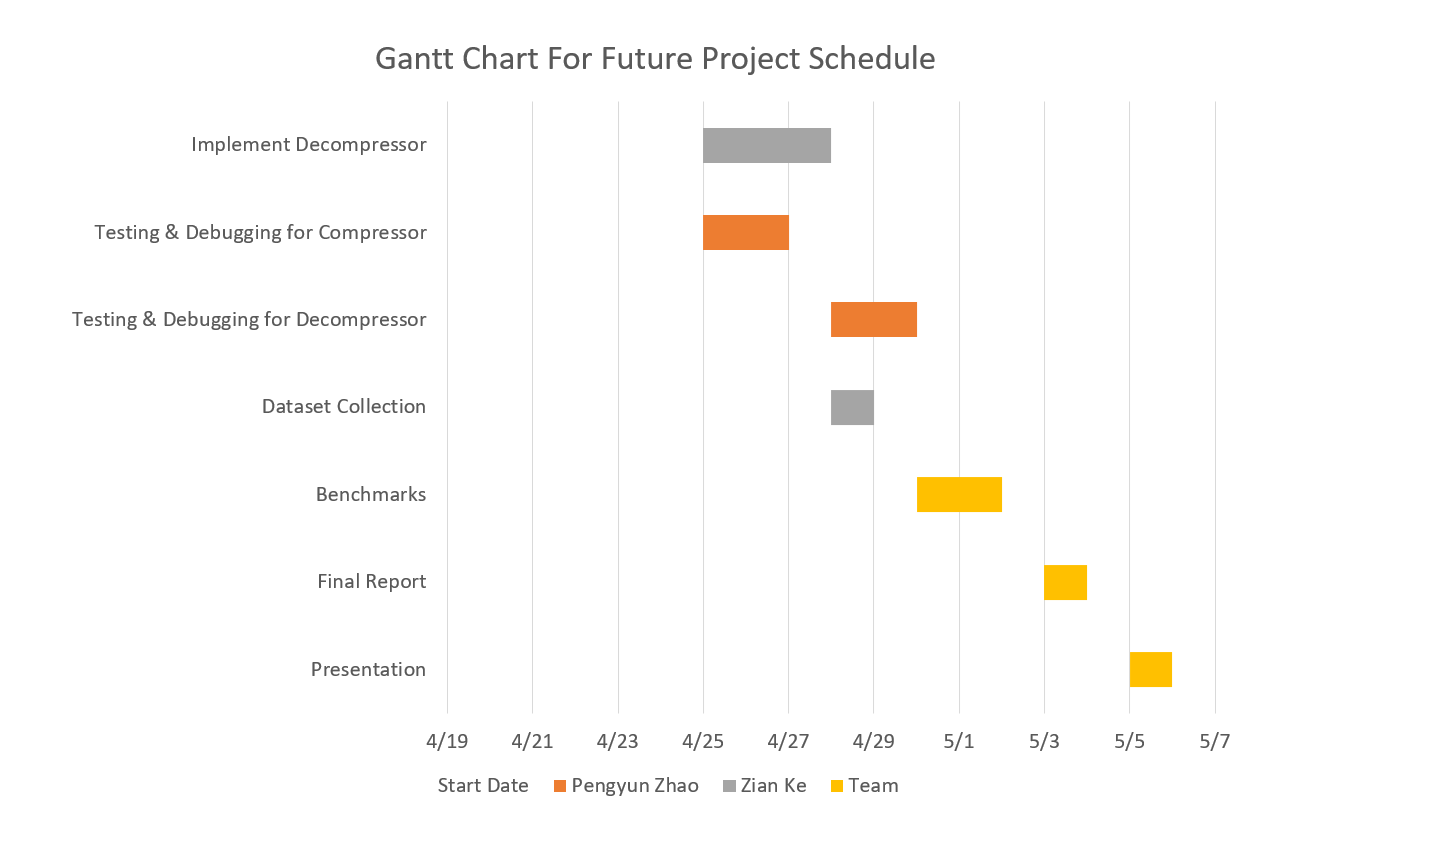
\includegraphics[width = 15cm]{gantt.png}
        \caption{Gantt Chart for Future Project Schedule}
    \end{center}
\end{figure}

\section{Deliverables}
Based on the fact that our current progress is going along quite well with our schedule, we think we will be able to achiveve the goals we plan to achieve stated in the project proposal. As for the ``nice to haves'', proving the efficiency and open source release are still challenging goals as they require a lot of work such as a diverse collection of datasets and use cases as well as detailed documentation and user support, but those goals are a good way to keep us motivated.

\noindent Also since now AWS is also offered as an option, we are interested in the program performance on different types of machines (GHC, Latedays, AWS) with different number and type of cores, and we want to include in the ``nice to haves'' in our goals.

\noindent So the new goals we plan to achieve are:
\begin{itemize}
    \item Implement a parallelized version of zlib in Go that produces correct compression and decompression results and is fully compatible with the standard Go zlib package, i.e.,  the data compressed by our parallel zlib can be decompressed by the standard zlib, and vice versa.
    \item Achieve noticeable speedup compared to the original sequential implementation.
    \item Have a comprehensive analysis on the implementation for different kinds of workloads. What are the new bottlenecks? What kind(s) of workload is suited for the parallel implementation?
\end{itemize}

\noindent Goals that we hope to achieve:
\begin{itemize}
    \item Achieve similar performance (or even better) with the currently released versions of parallel implementations.
    \item Prove the efficiency of parallel zlib in real-world applications such as large file compression and transport.
    \item Aim for open source release as a third-party Go package.
    \item \textbf{Analyze the program's performance on different machines. On which machines does the program have a higher performance, on which ones does it have a lower performance? What environment is it more suited for?}
\end{itemize}

\section{Presentation}
We plan to present a combination of demonstrations as well as charts and graphs.

\noindent Demonstrations are used to showcase the correctness of our program, i.e. it follows the zlib standard correctly and produces exactly same output (both decompression and compression).

\noindent Charts and graphs are used to represent the program's performance characteristics on different workloads and different machines and will help us present our analysis.

\section{Preliminary Results}
Based on our current implementation and testings, we have ensured that with a parallel zlib compressor that spawns multiple gorountines and compress multiple blocks concurrently, the correctness can still be guaranteed, i.e., the compressed result is fully compatible with a non-parallel zlib decompressor. We are also pretty sure that our parallel zlib compressor satisfies the requirement on \href{https://tools.ietf.org/html/rfc1950}{RFC 1950}, as we are strictly following the definitions of header,  checksum, etc., by taking the implementations of the standard zlib package in Go as reference.

\section{Issues}
A minor issue we currently have is about writing test cases. We planned to reuse the test cases in the standard zlib package in Go, as our implementation is expected to be compatible with it. However, those test cases have a dependency on the ``internal/testenv'' package, while Go does not allow third party packages to import internal packages. Hence we'll need to fully understand the standard zlib test cases and attempt to reimplement them, and also add more test cases, e.g., to test concurrency.

\end{document}

